\documentclass[12pt]{article}

\usepackage{fullpage}
\usepackage{graphicx, rotating, booktabs} 
\usepackage{times} 
\usepackage{natbib} 
\usepackage{indentfirst} 
\usepackage{setspace}
\usepackage{grffile} 
\usepackage{hyperref}
\usepackage{adjustbox}
\setcitestyle{aysep{}}


\singlespace
\title{
\textbf{Testing the Public Goods Theory of Alliances}
	}
\author{Joshua Alley\footnote{Graduate Student,
Department of Political Science, Texas A\&M University.}}
\date{{\normalsize \today}}

\bibliographystyle{apsr}

\begin{document}

\maketitle 

\doublespace

\begin{abstract}
\citet{OlsonZeckhauser1966}'s public goods model of alliances is influential but it has not subjected to careful empirical scrutiny. 
Prior studies suffer from an identification problem or only examined NATO. 
In this paper, I examine two predictions about alliance size and capability from the public goods model using more general and better-identified research designs. 
First, I test whether state size modifies the impact of increasing allied capability on growth in military spending. 
Then I estimate the association between treaty contribution and growth in military spending for 285 offensive and defensive alliances. 
Neither design supports the expectations of the public goods model. 
Therefore, the argument that alliances provide a public good and lead to free-riding should be treated with more skepticism. 

\end{abstract} 



%----------------------------------
\section{Introduction}



\citet{OlsonZeckhauser1966} argue that international alliances are subject to a collective action problem. 
Smaller alliance participants ``free ride'' on the contributions of larger members. 
This intuitive claim is quite influential. 


As of January 2019, Olson and Zeckhauser's article has 1684 citations.
Furthermore, they claim alliances are exemplars of collective action in international organizations. 
Given its salience and broad implications, this public goods theory of alliances merits careful scrutiny. 


But 52 years after the publication of ``An Economic Theory of Alliances,'' we have limited evidence for or against free-riding in alliances. 
The lack of reliable evidence is the consequence of two research design issues. 
First, many empirical models are unidentified.
Second, the overwhelming majority of tests focus on NATO. 


In this paper, I implement two tests the public goods model of alliances. 
Both tests correct the identification problem and broaden the scope of the analysis beyond NATO. 
I find little evidence for two predictions of the public goods model. 


Olson and Zeckhauser's measures of the defense burden and state size create an identification problem. 
They estimated correlations between military spending as a share of national income and national income.
This model is widely emulated, it places GDP on both sides of the equation.
Therefore, most empirical models of the public goods theory are unidentified.


Ratio dependent variables such as military expenditures as a share of GDP often generate spurious results \citep{Kronmal1993}. 
In Olson and Zeckhauser's test, changes in GDP impact the independent and dependent variable. 
There is a deterministic component in the relationship between GDP and the ratio of military expenditures to GDP. 


\citet{PluemperNeumayer2015} address the identification problem by examining changes in spending among NATO members. 
In their framework, unresponsiveness to US and Soviet military spending is evidence of free riding by non-US NATO members.
They find no correlation between the size of a NATO member and free-riding, which they argue contradicts Olson and Zeckhauser. 
However, they do not include the United States in their sample, which omits a crucial data point for testing the size argument.\footnote{Given the focus on responses to US spending, this decision is understandable.}


% So what is the problem here? 
The work of \citet{PluemperNeumayer2015} reflects the shortcoming of empirical tests of the public goods model of alliances.
Most studies focus on NATO, and we can conclude NATO members spend less on the military thanks to allied capability \citep{GeorgeSandler2017}.
But NATO is only one case. 


% by the way, it's mostly NATO
We do not know whether the public goods theory of alliances applies beyond NATO. 
My survey of the literature on alliance participation and military spending found six tests of the public goods theory of alliances outside of NATO. 
All six of those studies include GDP in the independent and dependent variable, creating an identification problem. 


% So it total, there's a lot we don't know
Despite the canonical status of \citet{OlsonZeckhauser1966}, their predictions have not been subjected to a general, well-identified test. 
Due to identification problems and emphasis on NATO, we have little evidence for the generalizability of the public goods theory of alliances.  
This failure to test the public goods theory of alliances well has two important consequences.

 
First, it hinders the accumulation of knowledge. 
Without a valid and comprehensive test, the explanatory power of the public goods theory of alliances is unclear. 
Other arguments that rely on the public goods conceptualization of alliances could rest on shaky empirical foundations. 


% Why we should care: policy and free riding
The public goods theory of alliances also has an outsized impact on policy. 
Charges of allied free-riding are ubiquitous in popular and policy debates. 
If the public goods theory of alliances makes inaccurate predictions, whether free-riding applies should be reassessed.


% I'm not the first one to address this theory: first comprehensive empirical evidence
Other scholars have questioned the public goods theory of alliances on theoretical grounds \citep{Palmer1990, SandlerHartley2001}.  
But theoretical revisions are premature without evidence a parsimonious public goods model is inappropriate. 
This paper provides the first comprehensive test of the public goods theory of alliances.  


Establishing the empirical validity of the public goods theory of alliances is crucial for academic theory and policy debates. 
Below, I outline two solutions to this challenge. 
Both research designs examine the role of alliance participant size in alliances from 1816 to 2007. 


The first design uses a conventional panel data model with an aggregate measure of alliance participation. 
I interact state size and changes in allied spending examine whether states reduce military expenditures as a result of increasing allied spending, and if reductions diminish with greater state size. 
The second design employs a Bayesian model to estimate the association between treaty contribution and growth in military spending for individual alliances. 
Neither approach finds evidence to match Olson and Zeckhauser's predictions. 


The paper proceeds as follows.
First, I summarize the public goods theory of alliances and two predictions of its logic.
Then, I describe the results of a panel-data test of the first prediction.
The third section tests the second prediction with a multilevel model. 
The final section assesses aggregate support for the public goods logic, as well as implications for scholarship and policy. 


\section{The Public Goods Theory of Alliances}

% this needs to be succint- aim for 500 words. 

% summarize argument
Why might alliances suffer from a public goods problem? 
The aggregate capability of an alliance provides security for members. 
Because a treaty cannot exclude members without undermining its purpose, security is a public good. 


Members gain security from treaty participation, regardless of their individual contribution. 
Olson and Zeckhauser expect that larger members of the alliance with bear a higher defense burden, because these states value defense from the alliance more. 
Smaller alliance members rely on the contributions of larger partners for security.
As a result, smaller states exploit larger alliance participants by free riding. 


% Develop implications for test: one for each section. 
There are two implications of this argument. 
Large and small states should respond differently to changes in allied military spending. 
If Olson and Zeckhauser's argument is correct, smaller states should decrease military spending in response to greater allied military spending. 
Larger states will be less responsive to increased allied spending. 
This implies a conditional relationship between allied spending, state size, and defense expenditures. 


\begin{quote}
\textsc{Hypothesis 1}: The marginal effect of allied spending on growth in military spending will be negative for small states, and increasing in state size. 
\end{quote}


The other prediction addresses individual alliance treaties. 
If larger states bear a disproportionate share of the alliance burden, then within each alliance, increasing contribution will require extra military spending. 
States that contribute more to the alliance will increase military expenditures to maintain security from the treaty. 


\begin{quote}
\textsc{Hypothesis 2}: Within an alliance, increasing treaty contribution will be positively associated with growth in military spending. 
\end{quote}


Treaties with a positive correlation between contribution and military spending match Olson and Zeckhauser's expectations. 
No correlation indicates larger members are not increasing military expenditures.
A negative correlation between treaty contribution and military spending implies larger members decrease spending. 


I now test these two predictions using an appropriate research design in a sample of all states except microstates from 1816 to 2007.\footnote{Including states with small GDP values makes estimating the interaction testing Hypothesis 1 difficult.}
The next section examines Hypothesis 1 by interacting changes in total allied spending and GDP.
This approach aggregates multiple treaties into a single measure of alliance participation. 


\section{Testing Hypothesis 1}

To test Hypothesis 1, I employ conventional measures of state size and alliance participation. 
Olson and Zeckhauser use GDP as a proxy for state size, so I constructed a measure of GDP using data from the Maddison Project \citep{Boltetal2018}. 
I then take the natural log of GDP to pull in outliers. 
I measure total allied capability as the military spending of all defensive or offensive alliance partners of a state.
All alliance membership data comes from the Alliance Treaty Obligations and Provisions (ATOP) dataset \citep{Leedsetal2002}.  


Growth in the natural log of military spending is the dependent variable \citep{SingerCINC1988}. 
The log-level of military spending is non-stationary.
Difference spending has changing variance over time, as budgets expand and generate larger changes. 
Modeling the DV in levels or changes with a control for the level might create spurious inferences \citep{GrangerNewbold1974}. 


Using growth in military spending as the dependent variable benchmarks changes to budget size. 
Change in spending occurs with reference to prior expenditures. 
This eliminates concerns with non-stationarity in changes or levels of military spending.
Growth in spending is equal to: 


\begin{equation}
\mbox{Growth Military Spending} = \frac{\mbox{Mil. Ex.}_t - \mbox{Mil. Ex.}_{t-1} }{ \mbox{Mil. Ex.}_{t-1} } = \frac{\Delta \mbox{Mil. Ex.} }{ \mbox{Mil. Ex.}_{t-1} }
\end{equation} 


Because Hypothesis 1 implies a conditional relationship, I interact allied spending and GDP in the following regression model:

\begin{equation} 
y = \beta_1 + \beta_2 \mbox{ln(GDP)} + \beta_3 \mbox{Ally Spend} + \beta_4 \mbox{ln(GDP)} \times \mbox{Ally Spend} + \beta \textbf{X} + \epsilon
\end{equation}


$\beta_2$ and $\beta_3$ are the constituent terms of the interaction and \textbf{$X$} is a matrix of control variables with coefficient vector $\beta$.
Hypothesis 1 implies $\beta_2$ should be positive, and $\beta_3$ should be negative. 
The interaction term $\beta_4$ should be positive. 


I estimate this model with a robust regression estimator. 
Growth in military spending has heavy-tailed residuals in a regression, so OLS is inefficient \citep{RaineyBaissa2018}. 
Robust regression re-weights observations using the size of the residual, making it less sensitive to large deviations than OLS. 


\textbf{$X$} contains correlates of alliance participation and military spending. 
I control for international war \citep{Reiteretal2016}, civil war participation \citep{SarkeesWayman2010}, and a count of annual MIDs \citep{Gibleretal2016}. 
Other controls average salient alliance characteristics, including democratic membership \citep{DigiuseppePoast2016} and number of members across a state's alliance treaties.   
Last, I control for regime type, external threat \citep{LeedsSavun2007}, and Cold War years. 


\subsection{Results}


Estimates from this model do not match the expectations of Hypothesis 1. 
\autoref{tab:rreg-res} summarizes results from the robust regression estimator. 
The log of GDP and changes in allied spending have no effect on growth in military spending. 
The interaction between changes in allied spending and GDP is also statistically insignificant. 


\begin{table}[!htbp] \centering 
  \caption{} 
  \label{} 
\begin{tabular}{@{\extracolsep{5pt}}lc} 
\\[-1.8ex]\hline 
\hline \\[-1.8ex] 
  & Growth Military Spending \\ 
\hline \\[-1.8ex] 
 Change Allied Spending & $-$0.026 \\ 
  & (0.047) \\ 
  & \\ 
 ln(GDP) & 0.0003 \\ 
  & (0.001) \\ 
  & \\ 
 Change Allied Spending $\times$ ln(GDP) & 0.002 \\ 
  & (0.002) \\ 
  & \\ 
 Avg. Alliance Size & 0.0003$^{*}$ \\ 
  & (0.0002) \\ 
  & \\ 
 Avg Alliance Democracy & $-$0.0003 \\ 
  & (0.001) \\ 
  & \\ 
 International War & 0.097$^{***}$ \\ 
  & (0.010) \\ 
  & \\ 
 Civil War Participant & 0.001 \\ 
  & (0.008) \\ 
  & \\ 
 POLITY & $-$0.0001 \\ 
  & (0.0004) \\ 
  & \\ 
 External Threat & 0.043$^{***}$ \\ 
  & (0.011) \\ 
  & \\ 
 Cold War & 0.047$^{***}$ \\ 
  & (0.004) \\ 
  & \\ 
 Constant & 0.026 \\ 
  & (0.030) \\ 
\hline \\[-1.8ex] 
Observations & 9,139 \\ 
Residual Std. Error & 0.157 (df = 9128) \\ 
\hline 
\hline \\[-1.8ex] 
\textit{Note:}  & \multicolumn{1}{r}{$^{*}$p$<$0.1; $^{**}$p$<$0.05; $^{***}$p$<$0.01} \\ 
\end{tabular} 
\caption{Robust Regression Estimates: Allied Spending, GDP, and Growth in military spending 1816-2007.}
\label{tab:rreg-res}
\end{table}


I cannot infer the absence of an interaction from the coefficients alone \citep{BramborClarkGolder2006}. 
\autoref{fig:abs-margins-plot} plots the marginal effect of allied military spending across the distribution of GDP. 
The marginal effect of allied military spending can only be distinguished from zero for positive values. 
There is no conditional relationship between state size and changes in allied spending. 


\begin{figure}
	\centering
		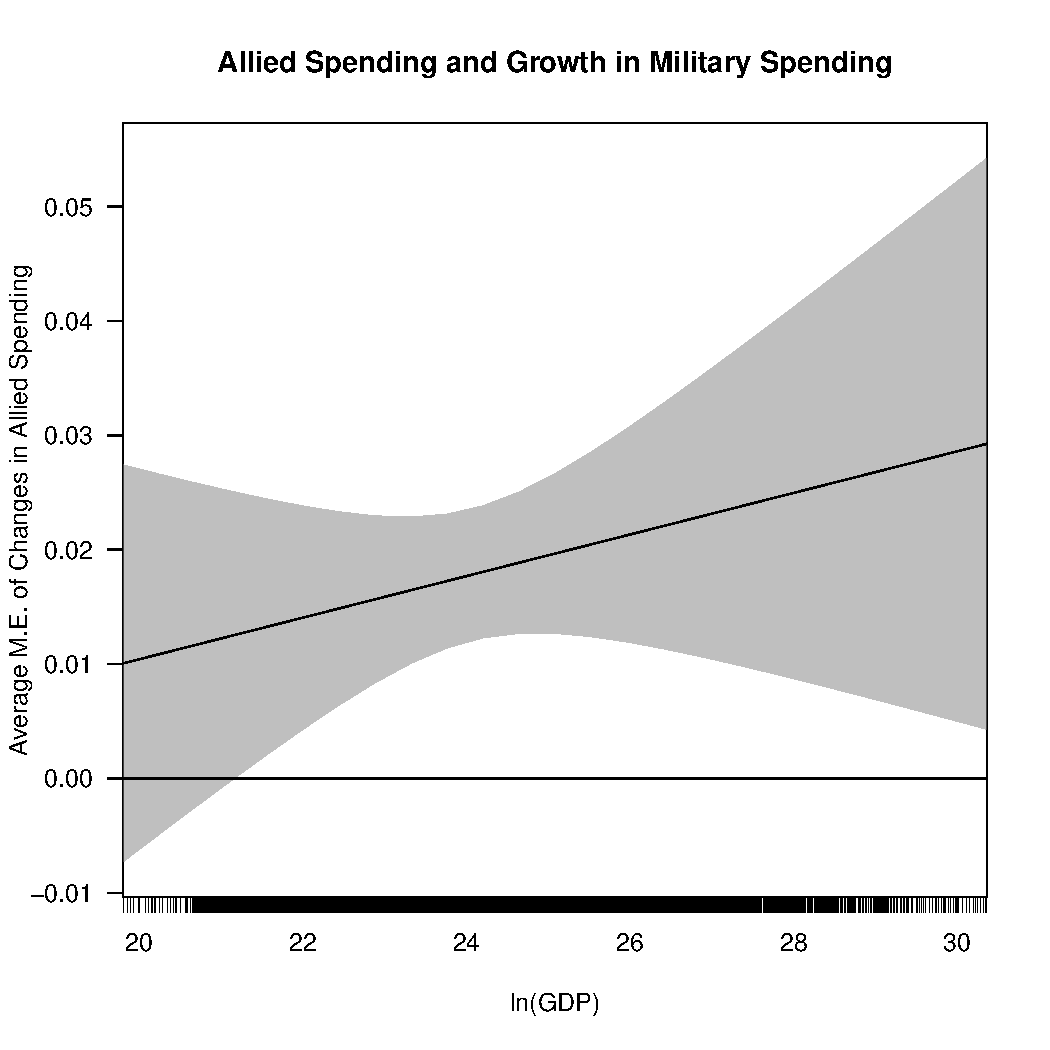
\includegraphics[width=0.95\textwidth]{abs-margins-plot.pdf}
	\caption{Average Marginal Effect of increasing allied military spending on a state's military spending, across the range of GDP.}
		\label{fig:abs-margins-plot}
\end{figure}


These results hold if I replace robust regression with OLS or employ kernel estimation of the interactive relationship \citep{Hainmuelleretal2019}.\footnote{See the appendix.} 
I also estimated a model using states with an alliance as the estimation sample with Heckman two-stage estimator to address non-random selection into alliances. 


This research design ignores heterogeneity among alliance treaties.
Olson and Zeckhauser focus on relative size, so states with small GDP can make large alliance contributions if their partner is even smaller. 
So the next section examines how many alliances have a positive correlation between treaty contribution and military expenditures. 


\section{Testing Hypothesis 2}


Testing Hypothesis 2 requires estimating the association between alliance contribution and military spending for each alliance.
For each of the 285 alliances that promise military support,\footnote{ATOP offensive and defensive treaties.} I estimate a parameter measuring the impact of increasing alliance contribution on military expenditures. 
Bayesian estimation regularizes estimates with hundreds of parameters, so I fit the following model using STAN \citep{Carpenteretal2016}.

The full model starts with state-year growth in military spending $y_{it}$.
I model the DV with a t-distribution to account for heavy tails.
$\nu$ is the degrees of freedom parameter--- as $\nu$ increases, the t distribution becomes more like a normal distribution. 


\begin{equation}
y_{it} \sim student_t(\nu, \mu, \sigma) 
\end{equation}


Most of this model follows standard panel data designs.
The expected value of the outcome $\mu_{it}$ depends on a constant $\alpha$, state and year varying intercepts $\alpha^{st}$ and $\alpha^{yr}$ and control variables $X_{it} \beta$. 
In this specification, I include all controls besides the alliance portfolio averages from the first robust regression in $X$.


\begin{equation}
\mu_{it} = \alpha + \alpha^{st} + \alpha^{yr} + X_{it} \beta + Z_{it} \gamma 
\end{equation}


The $Z_{it} \gamma$ term captures the impact of multiple alliances. 
\textbf{$Z$} is a matrix of state participation in alliances--- columns are alliances, rows are state-year observations. 
If a state is not in an alliance, the corresponding element of the matrix is equal to zero. 
If a state is part of an alliance, the corresponding element of the matrix is equal to a state's military spending as a share of total alliance expenditures. 
The alliance contribution elements of the matrix range from 0 to 1, because some states have no military spending.\footnote{Costa Rica is the best-known example of a state with no military spending.} 


$\gamma$ is a vector of 285 alliance-specific parameters.  
Because $Z$ contains alliance contribution, these coefficients estimate the association between treaty contribution and military spending. 
When a state is not in an alliance, the corresponding $\gamma$ is multiplied by zero, and has no impact. 
Alliance participation only affects military expenditures if a state contributes. 


Each alliance a state is a member of has a separate impact on military spending.
Thus, every alliance estimate holds the impact of other treaties constant. 
A positive $\gamma$ implies that as contribution to the alliance increases, members spend more, as Hypothesis 2 predicts. 
    


\subsection{Results} 


If the public goods theory of alliances is correct, we should observe many positive $\gamma$ parameters. 
Because I employed Bayesian modeling, each $\gamma$ has a posterior distribution.\footnote{See the appendix for a full summary of priors, convergence and model fit.} 
I focus interpretation on the posterior mean and 90\% credible intervals.\footnote{I use 90\% credible intervals because inferences around 95\% intervals can be less stable.}
The posterior mean is the expected value of $\gamma$, while the credible intervals capture uncertainty around that estimate.  


\begin{figure}[htbp]
	\centering
		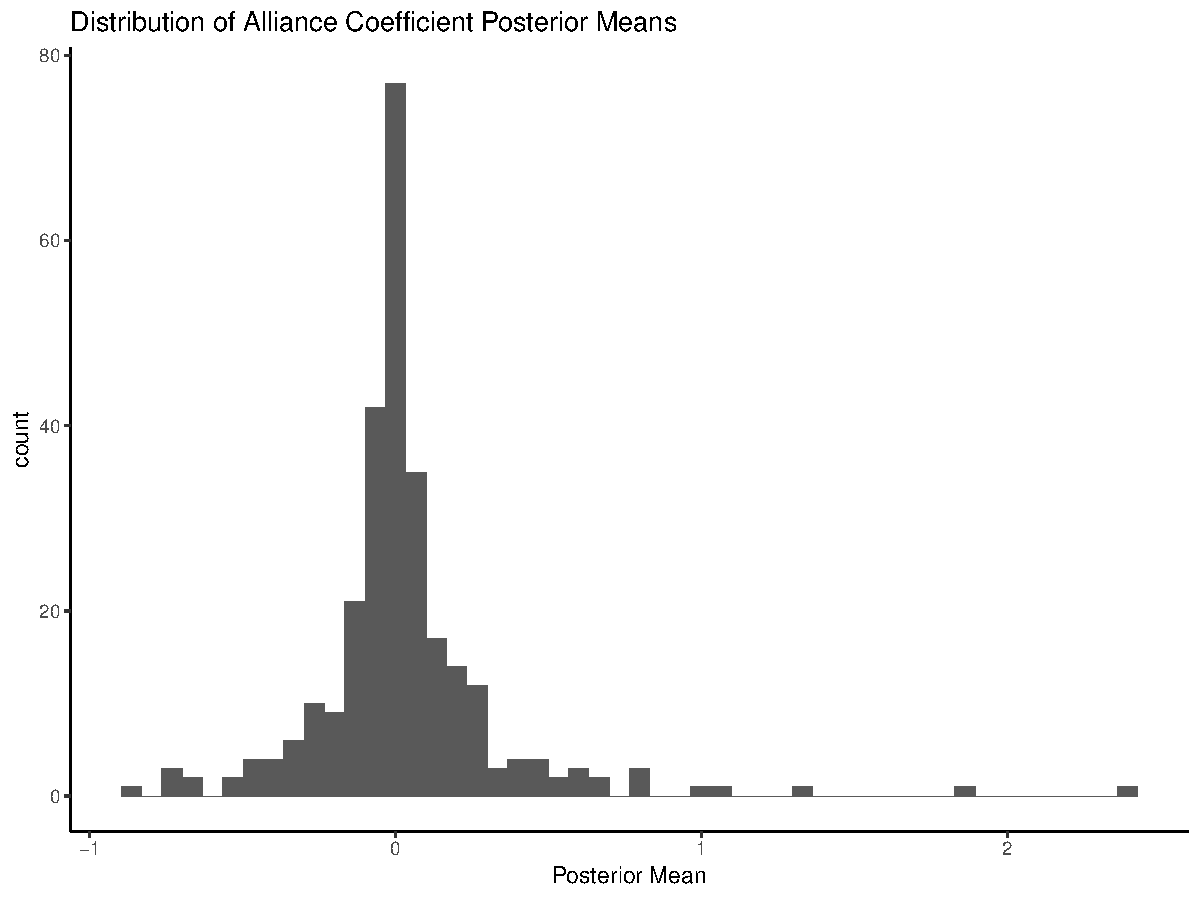
\includegraphics[width=0.95\textwidth]{alliance-coefs-hist.pdf}
	\caption{Posterior mean of association between alliance contribution and military spending in 285 defensive and offensive alliances from 1816 to 2007.}
	\label{fig:alliance-coefs-hist}
\end{figure}


\autoref{fig:alliance-coefs-hist} summarizes the posterior mean of the 285 alliance coefficients. 
Most means are close to zero. 
There are large positive values, but also many large negative values.


147 of 285 alliances have a positive posterior mean. 
138 of 285 alliances have a negative posterior mean. 
The large number of negative values is some evidence against Hypothesis 2. 
However, the posterior means do not convey whether the impact of increasing alliance contribution can be distinguished from zero. 


\autoref{fig:alliance-coefs-year} plots the $\gamma$ parameter for each alliance against the start year of the treaty.
Points mark the posterior mean. 
The error bars encapsulate the 90\% credible interval.\footnote{The credible interval falls between the 5\% and 95\% quantiles of the posterior.}  


\begin{figure}[htbp]
	\centering
		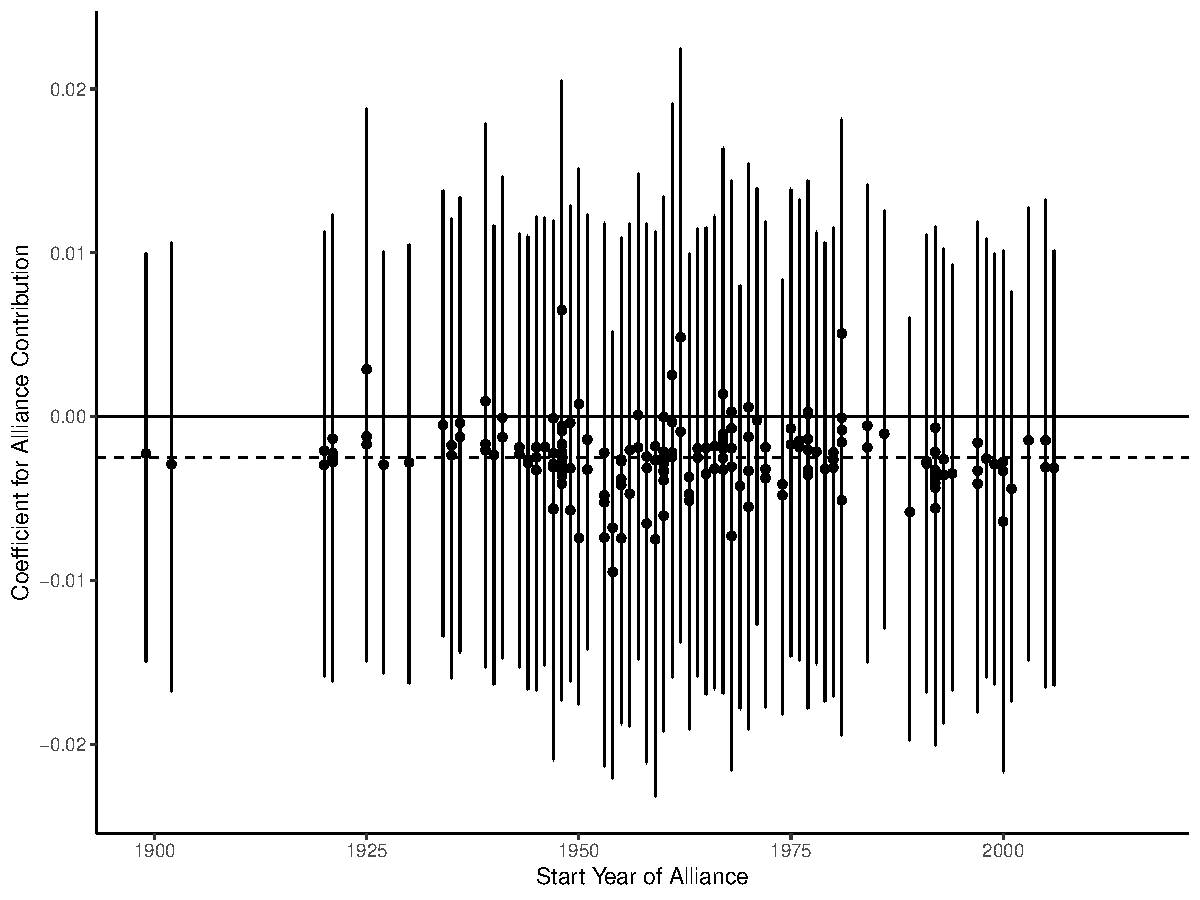
\includegraphics[width=0.95\textwidth]{alliance-coefs-year.pdf}
	\caption{Estimated association between alliance contribution and defense spending in 285 defensive and offensive alliances from 1816 to 2007. Points represent the posterior mean and the error bars cover the 90\% credible interval.}
	\label{fig:alliance-coefs-year}
\end{figure}


Most posterior means are close to zero, so 251 credible intervals include zero. 
There are 16 alliances where the credible interval includes only positive values, as the public goods model predicts. 
That leaves 13 treaties where the credible interval covers only negative values. 


16 of 285, or 6\%, is a dismal prediction success rate for Hypothesis 2. 
There is no association between treaty contribution and growth in military spending in most alliances.
The 13 negative $\gamma$ parameters imply larger members of those alliances \emph{lower growth in military spending}, which the public goods theory cannot explain. 


Alliances with a non-zero $\gamma$ provide additional information. 
We can look at these cases in more detail to look for free-riding. 
In \autoref{fig:nonzero-alliance-coefs}, I plot the posterior means of $\gamma$ for all 29 alliances.  
Several of these alliances have a large expected impact on military spending. 


\begin{figure}
	\centering
		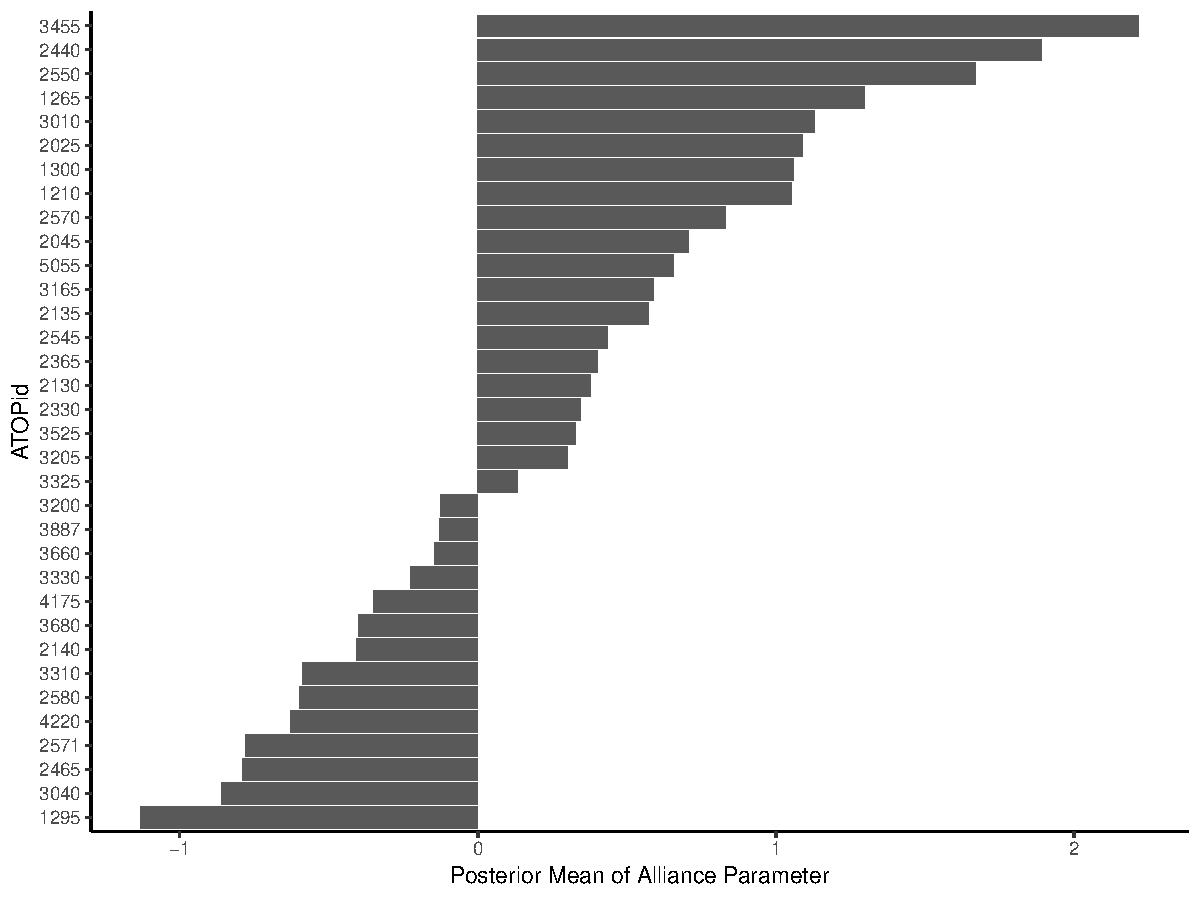
\includegraphics[width=0.95\textwidth]{nonzero-alliance-coefs.pdf}
	\caption{Bar plot of $\gamma$ for alliances where treaty contribution is positively or negatively correlated with military spending. The Y axis is the ATOP project's alliance identifier.}	
	\label{fig:nonzero-alliance-coefs}
\end{figure}


% Update this para. 
The largest positive association between treaty contribution and defense spending growth is the 1961 Defense Pact of the African and Malagasy Union (ATOPID 3455). 
The second largest is an 1866 offensive pact between Italy and Prussia (ATOPID 1265). 
Third largest is an Inter-American Hemispheric defense pact during World War II (ATOPID 3010). 


None of these three cases are obvious examples of free-riding. 
The Defense Pact of the African and Malagasy Union included most Francophone countries. 
The Union changed its functions to focus on economic affairs in 1964, dissolving the defense pact. 
Because the members of this treaty were geographically disparate and depended on France the defense functions of the treaty were weak from the start. 


The Italy-Prussia agreement and the Inter-American Hemispheric defense pact formed immediately before and during war, respectively. 
These treaties are a special cases in Olson and Zeckhauser's model where defense spending is a superior good--- increases in income are spent on defense. 
Larger members spent more because they used the treaty to expand their war-fighting efforts. 


Alliances with large negative $\gamma$ parameters have little in common with a public goods model. 
The largest negative association is an 1870 alliance between Prussia and the UK, signed during the Franco-Prussian war (ATOPID 1295). 
The second largest negative $\gamma$ is a June 1939 alliance between France and Turkey aimed at securing the Mediterranean (ATOPID 2465).
Last, the third most negative $\gamma$ is a 1944 agreement between the US and Portugal, where the Portuguese agreed to help in the Pacific theater. 


These three negative cases suggest states with resource constraints can use alliances to secure their interests and limit spending growth. 
Without a treaty with Prussia to guarantee Belgian neutrality, the UK would have spent more to defend Belgium in 1870.
France used the 1939 treaty with Turkey for similar purposes. 
The US formed the 1944 treaty with Portugal to further weaken Japan without exerting more military effort. 
These alliances structure particular exchanges among members, rather than provide some public good. 


NATO is the best example of collective defense, where other results suggest public goods dynamics are present. 
The estimated $\gamma$ for NATO offers no support for the public goods theory of alliances, however. 
The posterior mean is $-0.07$, and the credible interval ranges from -.30 to .14.  
Greater contribution to NATO is unassociated with growth in military spending. 
This finding corroborates the results of \citet{PluemperNeumayer2015}. 


A few cases may be subject to free-riding. 
The 2006 African Union Non-Aggression and Common Defense Pact (ATOPID 5055) has a positive $\gamma$ that might be explained by free-riding.  
China and North Korea's 1961 alliance (ATOPID 3445) is another possible example--- North Korea might have spent even more on the military without the Chinese alliance. 
Most of the other positive, non-zero $\gamma$ parameters are from treaties formed close to international conflict. 


This second set of estimates provides little support for predictions from the public goods theory of alliances. 
In 88\% of alliances, there is no association between treaty contribution and military spending. 
Even cases where treaty contribution is positively correlated with spending may not reflect collective action problems. 

%--- 
% Add discussion section given adequate space. 
%--- 


\section{Conclusion}

% Add paragraph summarizing results
Taking the results from testing Hypothesis 1 and 2 together, there is little evidence for the predictions of the public goods theory of alliances. 
There is no conditional relationship between GDP and changes in allied spending.
Moreover, there is a positive association between treaty contribution and military spending in only 6\% of alliances. 


These findings should increase our skepticism about the public goods model of alliances. 
Although Olson and Zeckhauser's model is simple and intuitive, it lacks explanatory power. 
Better identified empirical models and estimates from multiple treaties show little evidence small states leave larger counterparts to bear a higher burden. 


My results reinforce theoretical skepticism about the public goods model. 
\citet{Palmer1990} and \citet{SandlerHartley2001} provide two theoretical critiques that merit further attention. 
Constructing parsimonious models of alliances and defense effort is the next challenge for scholars. 
Components of the public goods model and these alternatives may provide a useful starting point. 


Some of the results raise additional questions for theoretical work. 
Why do we observe 14 alliances where increasing alliance contributions are associated with reduced spending?
Why is the effect of greater allied spending mostly positive in Model 1? 
Derivatives of the public goods theory may struggle to address these questions. 


Perhaps large and small states use alliances for distinct purposes, so members reap specific gains from treaty participation. 
Small states might use alliances to defend their homeland. 
Large states could be more focused on using alliances to defend other states and expand their influence abroad. 


Scholars and policymakers should reassess the idea of ``free-riding'' in alliance politics. 
Free-riding is inextricable from a public goods understanding of alliances.
But if key predictions of the public goods model have little empirical support, free-riding is an inaccurate description of reduced defense effort by alliance participants.  
Charges of free-riding are normatively loaded and may mask exchange between alliance members \citep{Lanoszka2015}. 


We should not completely abandon the public goods model in international politics. 
Other international organizations could be suffer from collective action problems.
International environmental regimes and climate change are one noteworthy example.  
Inferring collective action problems in other international organizations from alliances is inappropriate, however. 


Although influential, the public goods model of alliances has little explanatory power. 
I find little evidence that reduced military spending by alliance members is the result of a collective action problem. 
Few alliances provide public goods in a way that leads to the collective action problem envisaged by Olson and Zeckhauser. 



\singlespace


\bibliography{../../../MasterBibliography} 





\end{document}

